\section{Sistema de Refrigeração}
O sistema de refrigeração é uma etapa crucial do projeto da transportadora de órgãos, atendendo ao requisitos definidos o recipiente em que o órgão é armazenado e transportado deve se manter refrigerado durante o período de transporte. Refrigeração pode ser definida como todo processo de remoção de calor, redução e manutenção de temperatura de um espaço ou material abaixo da temperatura ambiente (JÚNIOR, 2003). Portanto, a partir da análise das características da demanda de refrigeração e do conhecimento para a construção e integração do produto, foram levantadas duas opções de resfriamento:
	\begin{itemize}
		\item Refrigeração Termoelétrica - Células Peltier;
		\item Refrigeração por Compressão Mecânica de Vapor - Compressor.
	\end{itemize}
	
	O refrigerador termoelétrico utiliza-se de dois materiais distintos, como pares termoelétricos convencionais. Há duas junções entre esses dois materiais em um refrigerador termoelétrico, uma está localizada no espaço refrigerado e a outra no meio ambiente. Quando se aplica uma diferença de potencial, a temperatura da junção que se encontra no espaço refrigerado diminui e a temperatura da outra junção aumenta. Operando em regime permanente, ocorrerá uma transmissão de calor do espaço refrigerado para a junção fria. A outra junção se encontrará a uma temperatura acima à ambiente e haverá, então, uma transmissão de calor para o local.
	
	A utilização dos módulos de peltier tem as seguintes vantagens: 
	
	\begin{itemize}
		\item Ausência de peças móveis e  gases refrigerantes  para refrigeração; 
		\item Aquece e resfria dependendo apenas da polaridade da alimentação;
		\item Ausência de barulho e vibrações;
		\item Tecnologia 100 por cento estado sólido; 
		\item Tamanho da solução reduzido e alta durabilidade;
		\item Funcionam em qualquer orientação com / sem gravidade diferente dos refrigeradores baseados em compressores.
		
	\end{itemize}
	
	Já o sistema de refrigeração por compressão mecânica de vapor funciona simplificadamente da seguinte forma: o fluido refrigerante que percorre um circuito fechado para absorver e remover o calor de um espaço que necessita de arrefecimento. Em qualquer processo de refrigeração, ocorre a transferência de calor de um ambiente para outro com a ajuda de um agente externo, que no caso deste sistema é o compressor (FERRAZ, 2008).
	
	Ao se optar por este tipo de sistema de refrigeração, têm-se como vantagens:
	\begin{itemize}
		\item Baixo consumo;
		\item Maior eficiência.
	\end{itemize}

	Em um primeiro momento optou-se pela refrigeração termoelétrica, realizaram-se vários testes de configurações para a célula peltier. Entretanto não foram obtidos resultados satisfatórios com relação à temperatura atingida dentro da câmara a ser refrigerada, apesar de conseguirmos uma temperatura adequada na face da módulo termoelétrico. A figura abaixo apresenta alguns dos testes realizados.
	
	
	\begin{figure}[H]
		\begin{center}
			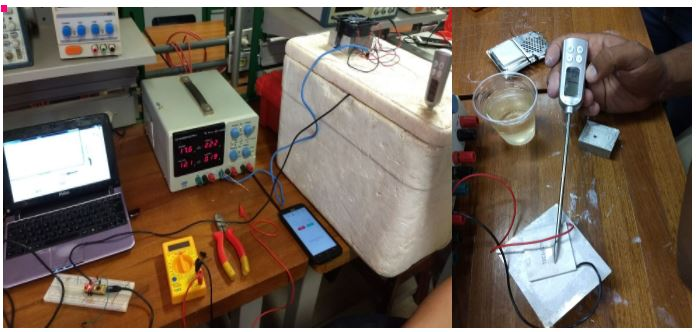
\includegraphics[scale = 0.8]{figuras/teste_Peltier.JPG}
			\caption{Testes iniciais utilizando a célula Peltier}
		\end{center}
	\end{figure}
	
	Devido aos resultados insatisfatórios, optou-se então pelo sistema por compressão mecânica de vapor, tendo como fonte de fornecimento uma bateria estacionária. O funcionamento do sistema de refrigeração construído está expresso na figura a seguir:
	\begin{figure}[H]
		\begin{center}
			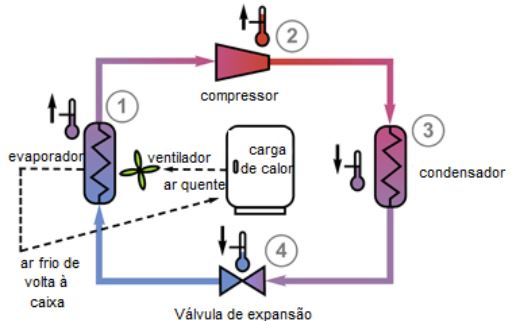
\includegraphics[scale = 0.75]{figuras/esquematico_compressor.JPG}
			\caption{Diagrama esquemático do sistema com compressor}
		\end{center}
	\end{figure}
	
	\subsection{Dimensionamento do Sistema}
		\subsubsection{Cálculo de Carga Térmica}
		Os cálculos da carga térmica objetivam determinar a quantidade de calor que deverá ser removida da caixa transportadora de órgãos, para que se atinja as condições adequadas para o armazenamento e transporte do órgão.
		
		Para desenvolver os cálculos da carga térmica do sistema, foram levantados os seguintes dados do sistema:
		\begin{enumerate}
			\item Dimensões da caixa interna (que contém o órgão):
				\begin{itemize}
					\item Altura: 0,2 m.
					\item Largura: 0,25 m.
					\item Profundidade: 0,25 m.
				\end{itemize}
			\item Dimensões da caixa externa:
				\begin{itemize}
					\item Altura: 0,3 m
					\item Largura: 0,3 m.
					\item Profundidade: 0,3 m.
				\end{itemize}
			\item Capacidade (volume) da caixa térmica: 0,0027 $m^3$ (27 L)
			\item Temperatura interna de operação: $2^oC$
			\item Temperatura externa à caixa:$ 35^oC$.
			\item Material de isolamento térmico: Poliestireno expandido.
			\item Espessura do material de isolamento térmico: 0,07 m.
			\item Tempo de resfriamento: 45 minutos.
		\end{enumerate}
		
		\subsubsection{Cálculo da energia e potência térmica do órgão:}
		Este cálculo se refere à quantidade de calor associada ao órgão e pode ser calculada pela equação:
		\begin{equation}
		Q = m \times c \times \Delta T
		\end{equation}
		
		Sendo: 
		$Q$ = energia térmica (KJ)
		
		$m$ = massa (g)
		
		$c$ = calor específico $(\frac{cal}{g^oC)}$
		
		$\Delta T$ = Variação da temperatura $(^oC)$
		
	Logo, a energia térmica do órgão é:
	$$
	Q_{órgão} = 13,8 KJ = 13,1 BTU
	$$	
	
	A potência térmica do órgão pode ser calculada a partir da equação a seguir:
	\begin{equation}
	P_{órgão} = \frac{Q_{órgão}}{\Delta t}
	\end{equation}
	Sendo:
	
	P = potência térmica (W);
	
	Q = energia térmica (KJ);
	
	$\Delta t$ = tempo de resfriamento (s)
	
	Logo, a potência térmica do órgão é:
	$$
	P_{órgão} = \frac{13,8}{\Delta t} \approx 5,1 W
	$$
	
	\subsubsection{Cálculo da energia e potência térmica da embalagem com solução Viaspan na qual o órgão está contido}
	Aplicando a equação para a energia térmica, tem-se:
	$$
	Q = 500  \times 0,97 \times 33 \approx 67 KJ \approx 63,5 BTU
	$$
	Aplicando a equação para a potência térmica, tem-se:
	$$
	P = \frac{67 KJ}{2700} \approx 24,8W
	$$
	
	\subsection{Cálculo da energia e potência térmica do alumínio da caixa interna}
	
	Aplicando a equação para a energia térmica, tem-se:
	$$
	Q_{aluminio} = 3000g \times 0,22\frac{cal}{g ^oC} \times 33 \approx 91,2 KJ \approx 86,4 BTU
	$$
	
	Aplicando a equação para a potência térmica, tem-se:
	$$
	P_{aluminio} = \frac{91,2 (KJ)}{2700 s} \approx 33,8 W
	$$
	
		A soma das potências térmicas do órgão, da embalagem contendo a solução Viaspan e do alumínio fornecem a potência térmica total do interior da caixa, necessária ao resfriamento, como mostra a equação a seguir:
		$$
		P_{interna} = P_{órgão}
 + P + P_{Alumínio}		$$
 
		 $$
		 P_{interna}(W) = 5,1+24,8+33,8 = 63,7 W
		 $$
		A caixa externa também está envolvida nos cálculos de potência térmica devido à transferência de calor que ocorre entre a vizinhança e o sistema.
		
		\subsubsection{Cálculo da resistência térmica $(Rt)$ e o coeficiente global de transferência de calor (U)}
		
		A resistência térmica é calculada a partir da equação:
		
		$$
		R_t = \frac{L_{isopor}}{K_{isopor}}
		$$
	
	Sendo:
	$R_t$ = resistência térmica $\frac{m^2K}{W}$
	
	L = espessura (m)
	
	K = condutibilidade térmica $\frac{W}{mK}$
	
	Aplicando a equação, tem-se:
	$$
	R_t = \frac{0,7}{0,007} = 2\frac{m^2K}{W}
	$$
	
	O coeficiente global de transferência de calor é calculado a partir da equação.
	\begin{equation}
	U = \frac{1}{R_t}
	\end{equation}
	Aplicando a equação acima, tem-se:

	$$
	U = \frac{1}{2} = 0,5 \frac{W}{m^2 K}
	$$
	
	A quantidade de calor que atravessa as paredes da caixa externa é dada pela equação a seguir:
	\begin{equation}
	Q = U \times A \times \Delta T
	\end{equation}
	
	Sendo:
	
	
	Aplicando a equação, considerando-se a área total da caixa, tem-se:
	Q = quantidade de calor que atravessa a parede da caixa (W);
	
	A = área da parede ($m^2$);
	
	U = coeficiente global de transferência de calor ($\frac{W}{m^2K}$)
	
	$\Delta T$= variação da temperatura (ºC)
	
	Como a área da parede é dada por $A = 0,09 m^2 \times 6$, temos a seguinte relação:
	$$
	Q = 0,5 \times 0,54 \times 33K \approx 8,91 W
	$$
	Por fim, a potência térmica total do sistema é calculada pela soma da potência térmica interna da caixa junto a quantidade de calor que atravessa as paredes da caixa externa.
	$$
	P_{total} = P_{interna} + Q \longrightarrow P_{total} \approx 63,7 + 8,91 \approx 72,61W
	$$
	
	Desta forma, conclui-se que o sistema de refrigeração deve suprir a potência de 72,61 W para o resfriamento às condições desejadas.
	
	\subsection{Evaporador}
	Para determinar a área do trocador de calor, podemos utilizar o Método de  Média Logarítmica das Diferenças de Temperatura que é dado pela seguinte relação:
	
	\begin{equation}
	Q = k \times A \times \Delta T_{ln}
	\end{equation}
	
	Onde:
	
	Q - taxa de transferência térmica 
	
	K - coeficiente de transferência de calor global
	
	A - área de superfície de transferência de calor
	
	$\Delta T_{ln}$ - diferença de temperatura média logarítmica (K)
	
	Utilizando as seguintes determinações para as temperaturas:
	
	\textit{Fluido quente(Ar)}: $T_e$= $25^oC$    e     $T_S$= $2^oC$
	
	
Como o valor do coeficiente global de transferência de calor (K) pode variar, conforme a tabela abaixo,
	\begin{figure}[H]
	\begin{center}
	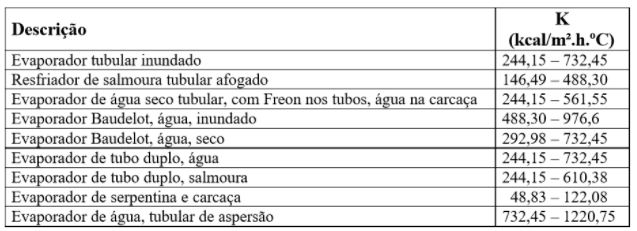
\includegraphics[scale =1]{figuras/Tabela_K}
	\caption{Tabela com os possíveis valores de K}
	\end{center}
	\end{figure}
	
	e considerando o pior dos casos de transferência de calor, obtemos um valor de 48,83 $\frac{kcal}{m^2\times h \times ^oC}$ para um evaporador de serpentina e carcaça, que é o nosso caso.
	
	Formulando, obtemos a seguinte equação:
	$$
	Q = K \times A \times \frac{\Delta T_S - \Delta T_e}{ln\left(\frac{\Delta T_s}{Delta T_e}\right)}
	$$
	
	De forma que se obtém:
	
	$$
	72,61 = 48,83 \times A \times \frac{2 - 35}{ln\left(\frac{2}{35}\right)}
	$$
	
	Como $A = \pi \times D \times L$ e D = 0,007 m, é possível encontrar L = 5,7 m.
	 
	A capacidade frigorífica ($Q_0$) é a quantidade de calor por unidade de tempo retirada do meio que se quer resfriar (produto) através do evaporador do sistema frigorífico. Para o sistema operando em regime permanente desprezando-se a variação de energia e potencial, pela primeira lei da termodinâmica obtém-se: 
	
	\begin{equation}
	Q=m_f \times (h_1-h_4)
	\end{equation}

	\begin{figure}[H]
		\begin{center}
			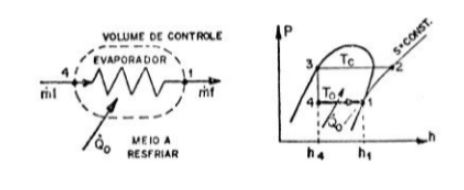
\includegraphics[scale =1]{figuras/Volume_Evaporador}
			\caption{Volume de controle aplicado ao evaporador e a indicação do processo }
		\end{center}
	\end{figure}
	
	$Q_0$ é a capacidade frigorífica  do ciclo operando em temperaturas $TC$ e $T_0$ para $m_f$, entalpia específica $h_1$ e  $h_4$. O fluxo de massa de refrigerante (mf) deve ser mantido pelo compressor. Normalmente se conhece a capacidade frigorífica que deve ter o sistema de refrigeração, que deve ser igualada à carga térmica, se estabelecermos o ciclo de refrigeração que deve operar o sistema podendo assim determinar o fluxo de massa e, consequentemente, o compressor necessário ao sistema (JÚNIOR, 2005).
	
	 A quantidade de calor retirado por um quilo de refrigerante através do evaporador é denominada “Efeito Frigorífico - E.F.”, isto é :
	 \begin{equation}
	 EF = h_1-h_4
	 \end{equation}
	 Sendo, $T_C$= $30^oC$ e $T_0$ = $22^oC$, para o gás refrigerante R134a, obtemos  $h_1$ =180,5  kJkg  e $h_4$ = 173,1 kJkg  , logo
	 
	 $$
	 E.F = 180,5 - 173,1 = 7,4
	 $$
	 
	 Então, substituindo pelos dados coletados:
	 
	 $$
	72,61 =m_f \times 7,4 \longrightarrow m_f=9,81 \frac{Kg}{h}
	 $$
	 \subsection{Compressor}
	 Para o dimensionamento do compressor, é necessário calcular a potência necessária para fazer o fluido refrigerante circular pela serpentina. Essa potência foi encontrada a partir da formulação: 
	 
	 \begin{equation}
	 W_c = m_f \times (h_2 - h_1)
	 \end{equation}
	 
	 Sendo:
	$ W_c$ -  potência teórica do compressor); 
	
	 $m_f$ - fluxo de massa refrigerante;
	 
	 $h_2$ -  entalpia no início da compressão;
	 
	 $h_1$ - entalpia no final da compressão;
	 
	 $$
	 W_c = 9,81 \times (194,8 - 180,5) \approx 140,28
	 $$
	 
	 \section{Estrutura do Conjunto de Refrigeração}
	 Após o dimensionamento do Sistema de Refrigeração, ocorreu a montagem do sistema final. O sistema dimensionado foi acoplado a estrutura geral do projeto, conforme demonstrado na Figura abaixo
	 	\begin{figure}[H]
	 		\begin{center}
	 			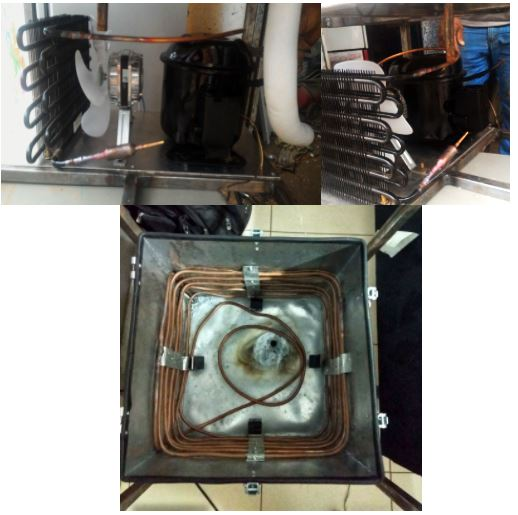
\includegraphics[scale =1]{figuras/Estrutura_refrigeracao}
	 			\caption{Estrutura do sistema de refrigeração }
	 		\end{center}
	 	\end{figure}
	 O compressor escolhido que satisfazia todas as necessidades dimensionadas, possui as seguintes especificações:
	 
	 	 	\begin{figure}[H]
	 	 		\begin{center}
	 	 			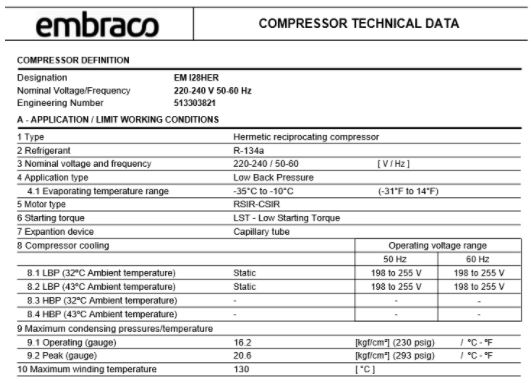
\includegraphics[scale =1]{figuras/caracteristicas}
	 	 			\caption{Especificações Técnicas do Compressor.
	 	 				 }
	 	 		\end{center}
	 	 	\end{figure}
	 	
\section{Sistema de Alimentação}
As fontes de energia que serão utilizadas para alimentar o produto, incluindo o sistema de refrigeração e os componentes elétricos e eletrônicos, são a rede elétrica comum brasileira e um banco de baterias. O banco de baterias será dimensionada a fim de manter os subsistemas em perfeita operação durante o período solicitado de 48 horas.

\subsection{Diagrama do Sistema}
A Figura a seguir apresenta o diagrama elétrico simplificado do produto. Ele representa o circuito de alimentação utilizado, desde a fonte de energia --- rede elétrica padrão --- até o uso final em seus componentes elétricos e eletrônicos.

\begin{figure}[H]
\begin{center}
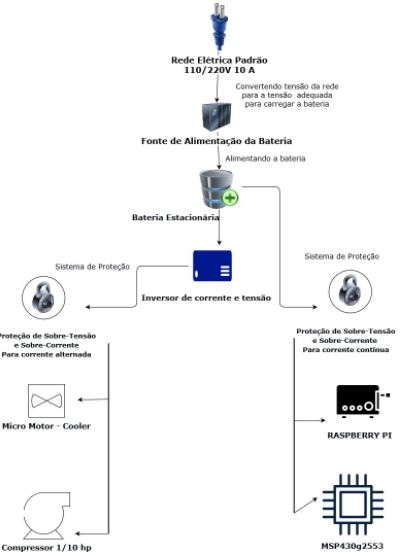
\includegraphics[scale = 1.2]{figuras/Diagrama_Simp.JPG}
\caption{ Diagrama Elétrico Preliminar}
\end{center}
\end{figure}

O sistema foi dimensionado com um fator de segurança elevado, pois a proposta de projeto é de um sistema de acondicionamento de órgãos para transplante. Sendo assim, o nível de confiabilidade do produto deve ser extremamente alto, para isso todo o sistema de alimentação foi dimensionado relacionando o sistema ao tempo de operação necessário ao transporte e diretamente ao consumo de energia advinda da bateria.

\subsection{Sistema de proteção de componentes elétricos e eletrônicos}
Devido ao grau de confiabilidade que o produto construído demanda, por ser um sistema de transporte de órgãos para transplante, têm-se que instalar diversos circuitos de proteção de componentes, garantindo assim o perfeito estado e funcionamento dos componentes internos.

Para isso foi utilizado um circuito de proteção contra sobretensão com base em um SRC ou diodo controlado de silício. Este componente é muito importante em aplicações que possuem o objetivo de controlar cargas de potência de altos valores a partir da rede de energia.

Sendo assim, desenvolveu-se uma topologia de circuito utilizando o regulador de tensão LM7805 para estabilizar em 5Vdc e utilizar um diodo zener de proteção para estabilizar a tensão abaixo de 5.1Vdc. Caso ocorra uma sobrecarga de tensão no circuito, o diodo zener passará a conduzir corrente acionando os 2 SRCs e consequentemente queimando o fusível de proteção.

Pode-se observar na imagem abaixo o esquemático do circuito a ser implementado:

	\begin{figure}[H]
		\begin{center}
		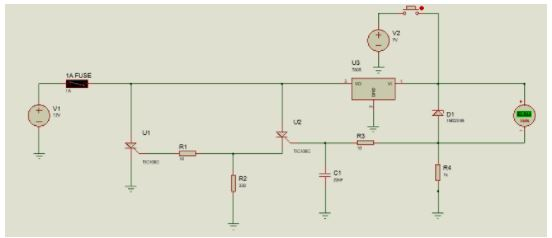
\includegraphics[scale = 1]{figuras/Circuito_Protecao}
		\caption{Circuito de proteção}
		\end{center}
	\end{figure}
Neste caso, pode-se observar uma fonte de 7V acoplada a um botão que simula uma sobretensão, 2 SRCs que são ativados quando o zener sobre uma sobretensão  causando a abertura do SRC U1 e consequentemente ativando o fusível. Desta forma,  garantimos  a proteção dos componentes, o diodo zener funciona como um sensor de corrente, caso a tensão ultrapasse os 5.1 V, o diodo passará a conduzir corrente, ativando a base do transistor quando essa corrente chegar a 10mA, abrindo o circuito e consequentemente acionando o fusível.

Após a simulação, foram realizados testes de prototipagem em protoboard. Em seguida, depois da verificação da funcionalidade do sistema a nível de prototipagem, foi dimensionado o layout do circuito para realizar a confecção da PCB por meio de serigrafia e corrosão no percloreto de ferro. A seguir, ilustram-se o layout da placa e o circuito já impresso.


Por fim foram realizados testes utilizando uma fonte de bancada e setando sua entrada em 12 V DC, neste caso foi observada  uma saída de 5.1V suficiente para alimentar tanto a raspberry PI quanto o MSP430

	\begin{figure}[H]
		\begin{center}
			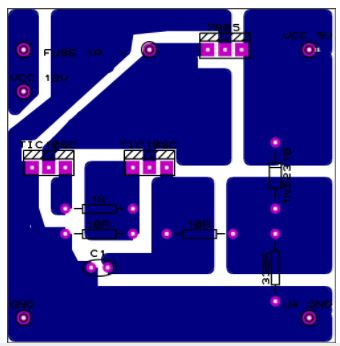
\includegraphics[scale = 1]{figuras/Layout_Protecao}
			\caption{Layout do circuito de proteção}
		\end{center}
	\end{figure}
	
		\begin{figure}[H]
			\begin{center}
				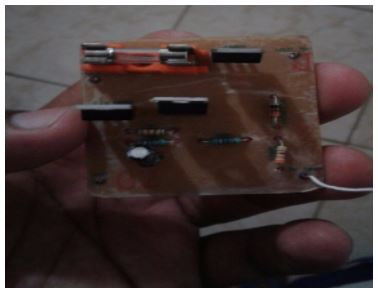
\includegraphics[scale = 1]{figuras/Circuito_Impresso}
				\caption{Circuito de proteção impresso}
			\end{center}
		\end{figure}
\subsection{Baterias}
	Baterias têm a finalidade de armazenar energia e liberá-la em determinada periodicidade, e de forma controlada. Sua escolha deve ser adequada às necessidades de consumo energético do projeto, e considera os dados de corrente elétrica e tensão. Para a seleção da bateria adequada deve-se estudar se ela é capaz de armazenar a energia total demandada às necessidades do projeto, e se ela consegue entregar toda a energia necessária ao funcionamento do equipamento. O processo de dimensionamento do banco de baterias deve ser realizado inicialmente e depois sucessivamente aperfeiçoado, em função dos demais dimensionamentos e ajustado em função dos custos, disponibilidade de mercado, entre outros.

	O processo de dimensionamento deve seguir algumas etapas, a primeira delas é definir o tipo de bateria a ser utilizado. Dentre as opções de bateria disponíveis no mercado, optou-se pela bateria estacionária. Sua vida útil é de aproximadamente 5 anos, devido à sua composição com materiais internos mais sobres se comparada às baterias automotivas, por exemplo. Podem, também, suportar descargas de até 80\% de sua capacidade, sem prejudicar sua vida útil, e resistem a ciclos de carga ou descarga mais profundos. Tais características proporcionam maior confiabilidade ao funcionamento do projeto pelo uso da bateria estacionaria.
	
	Após a escolha do tipo de bateria, deve ser analisada a profundidade de descarga com que se vai trabalhar. Quanto mais profundos os ciclos de descarga-carga, menor a vida útil da bateria. Ou seja, reduzir-se a capacidade da bateria, gasta-se menos no início, porém as baterias durarão menos e os gastos com reposição serão maiores. Um valor usado para essa profundidade de descarga para ciclos diários com baterias de chumbo-ácido é de 10\% a 20\%. Para ciclos esporádicos, podem ser utilizados ciclos mais profundos, da ordem de 60\%. 
	
	A capacidade do banco de baterias em Ah pode ser calculada conforme a expressão abaixo: 
	
	\begin{equation}
	Capacidade(Ah) = \frac{Consumo(\frac{Wh}{dia}) \times Autonomia(dias)}{V_{Baterias}(V)\times profundidade(pu)}
	\end{equation}

O dimensionamento da bateria requer inicialmente a relação de potência demandada para suprir as necessidades dos componentes elétricos do projeto, como mostra a tabela a seguir:

\begin{table}[H]
\caption{Consumo energético dos componentes}
\begin{tabular}{|p{4 cm} |c |c |c |}
 \hline
   \textbf{COMPONENTE} &\textbf{ALIMENTAÇÃO (V)}  &\textbf{CORRENTE (A)} & \textbf{POTÊNCIA (W)} \\
   \hline
  \textbf{Microcontroladores} &5 & 240$\mu$& 1,65 mW \\
   \hline
   \textbf{RASPBERRY PI}&5 &2,5 & 12,5 \\
   \hline
  \textbf{PROTETOR } &12 &26,5m &318m \\
   \hline
  \textbf{COMPRESSOR $\frac{1}{10}HP$} &12 & 2,4& 28,33 \\
   \hline
  \textbf{MICRO MOTOR} &12 &260,9m &3,6  \\
   \hline
	\textbf{INVERSOR GIGAL (stabd by)} &12 &400m &4,8  \\
	\hline
\end{tabular}
\end{table}

Ao somar todas as cargas necessárias, o total foi de 229,819 Wh, já o consumo de corrente fica em 3,5365 A/h. O principal problema é o alto valor de partida do motor-compressor, o que é chamado de corrente de pico, no caso do motor-compressor utilizado, a corrente pode atingir um o valor entre 2-3 Ampères, o que requer atenção ao dimensionar a bateria para que ela suporte esse aumento inicial.


Com relação a profundidade da descarga no final da autonomia (pu) - utilizamos 0,6 (descargas mais profundas significam vida útil menor para a bateria e menos profundas um investimento inicial maior). Sendo que o consumo total é obtido a partir do levantamento das cargas, a autonomia de 5 horas.

Logo, 
$$
Capacidade \approx 33,2439 Ah
$$
\subsection{Partida de Motor Compressor}
Os motores de indução monofásicos,como é o caso de um compressor, são aplicáveis em sistemas que são alimentados diretamente por uma fonte monofásica. São vários os tipos desses motores, e suas aplicações dependem basicamente do tipo de sistema a ser acionado. No caso da transportadora de órgãos, foi utilizado um motor de indução monofásico de potência de 1/10 HP.

No momento do acionamento de um motor de indução, este se comporta como um transformador, em que o enrolamento secundário corresponde ao do rotor parado e curtocircuitado. Como o circuito do rotor apresenta uma baixa impedância, têm-se um alto valor de corrente induzida no enrolamento do secundário que se reflete para o circuito do estator que está conectado diretamente à fonte de alimentação em tensão nominal. Sendo assim, em alguns casos um motor de indução requer aproximadamente seis vezes a sua corrente nominal para a partida a tensão nominal.

Essa alta corrente de partida de motores de indução  pode ocasionar alguns problemas como a queda de tensão na rede de alimentação, o aumento da bitola dos condutores de alimentação e a necessidade de transformadores de maior potência. O que dificulta a partida por meio de um método que não seja o de ligação direta à rede, sem que se verifiquem quedas na tensão de suprimento e sem um grande aumento do período de aceleração, desde o repouso até o alcance da velocidade nominal. Portanto, deve-se dispor de algum tipo de dispositivo que limite a corrente de partida.

\subsection{Dimmer Microcontrolado}
 A partida direta no motor de indução de 1/10de HP gera uma corrente de pico de 4.8A (valor obtido experimentalmente com alicate amperimetro MINIPA), essa exige uma corrente no primário do transformador de aproximadamente 88A desprezando as perdas por corrente de focault e as perdas por efeito Joule no aquecimento dos fios.
 
 Por este motivo  foi escolhido utilizar a partida em rampa, sendo esta aplicado por um dimmer microcontrolado, realizando o controle de potência AC. Desta forma, pode-se variar a potência de entrada para que a partida seja mais suave, ou seja, uma entrada em rampa diferentemente do Degrau, diminuindo a corrente de pico do regime transiente e consequentemente demandando menor esforço e potência de pico pelo inversor.
 
 A fim de detectar a passagem por 0 e disparar um pulso para o microcontrolador foi inserida uma ponte retificadora para rebater a onda e torná-la positiva,  fazendo com que a passagem por 0 seja de possível detecção por um microcontrolador através de um circuito optoacoplador. Foi escolhido o chip optoacoplador 4N25 para que fosse possível detectar a passagem por fase 0, pela sua característica de emissão de luz suficiente para  polarizar o gate do fototransistor a partir de uma tensão senoidal de 10Vpp ou superior.
 
 A saída do do fototransistor foi ligada a um resistor de pull-up e conectada ao microcontrolador, para que assim seja detectada a passagem por 0 para então disparar o fototriac.
 
 Para controlar através do microcontrolador, é necessário um circuito de isolamento do circuito de baixa tensão para com o circuito de alta tensão, por isso utilizamos um fototriac MOC3021 que é capaz de ser acionado através de uma tensão de entrada da ordem de 3.3V, tensão de saída do próprio microcontrolador para realizar o disparo do pulso que controla a passagem da onda através do triac.
 
 Com base nessas capacidades do Triac, o microcontrolador desliga brevemente a tensão da rede, durante uma parte de cada um dos ciclos. Isso acontece 120 vezes por segundo (ou 2 vezes por ciclo), causando apenas uma redução da potência, equivalente à que acontece quando há uma queda de tensão da rede elétrica, embora causada por outro princípio (o mecanismo aqui descrito não modifica a tensão, apenas o tempo durante o qual ela fica disponível).
 
O gráfico a seguir mostra o que acontece durante cada um dos ciclos AC (ou seja: a senóide apresentada se repete 60 vezes por segundo):

		\begin{figure}[H]
			\begin{center}
				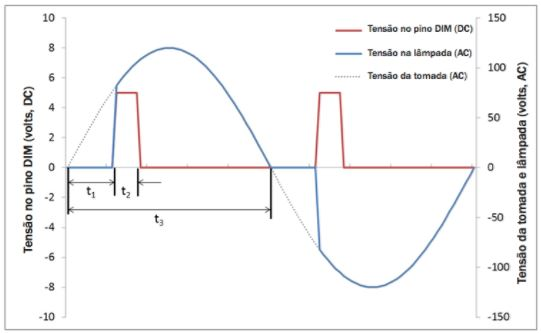
\includegraphics[scale = 1]{figuras/Grafico_Dimmer}
				\caption{Exemplo de circuito dimmer entrada , pulso e saída.}
			\end{center}
		\end{figure}

O eixo X é o tempo, e o gráfico inteiro se repete 60 vezes por segundo, ou seja, a linha horizontal representada no gráfico equivale a 1/60 de segundo.

Note que o eixo Y tem 2 escalas: a da esquerda, de -10V a +10V, vale apenas para a linha vermelha, que indica a tensão ativada pelo microcontrolador no pino DIM do módulo, e a da direita, que vai de -150V a +150V, e vale para a linha pontilhada (que indica a tensão recebida da tomada pelo módulo) e para a linha azul (que indica a tensão fornecida à lâmpada pelo módulo).

A linha pontilhada é visível apenas em 2 pequenos trechos, porque nos demais ela é sobreposta pela linha azul.

A linha vermelha geralmente está fixa em 0 volts, exceto em 2 breves momentos, que ocorrem após o tempo t1 (que começa a contar sempre que a tensão da tomada passa pelo 0V) e cuja duração equivale ao tempo t2, que correspondem aos pulsos positivos (HIGH) que o microcontrolador envia para o pino DIM do nosso módulo, indicando que ele pode liberar a passagem entre a tomada e a lâmpada.

Note também que, no mesmo momento em que a linha vermelha começa a estar HIGH, a linha azul passa de 0V para o mesmo valor da tensão recebida da tomada (linha pontilhada) naquele momento: é o momento em que a lâmpada acende.

Foi realizado o cálculo, com base no valor da variável volátil potência (que deve variar entre 0 e 100), qual será a duração do tempo t1 - quanto menor a potência desejada, maior deve ser o tempo t1, até um limite próximo a 1/160 de segundos, ou aproximadamente 8333 microssegundos.

Foi utilizado o valor de  8200 (e não 8333) como o limite máximo, para evitar que a soma de t1 + t2 (mais o tempo que leva para executar os comandos da zeroCross()) ultrapasse os 8333 microsegundos que temos entre cada chamada. O valor de  t2 ficou fixado (logo abaixo) em 6 microssegundos.

Com t1 e t2 definidos nos registradores a seguinte sequencia é seguida:

\begin{itemize}
	\item Aguardar t1 microssegundos;
	\item Mover HIGH para o pino DIM;
	\item Aguardar t2 microssegundos;
	\item Mover LOW para o pino DIM
\end{itemize}

E assim termina a função zeroCross(). Com isso, a interrupção INT0 se encerra (até que outra aconteça), e a execução retorna ao ponto em que o programa "normal" foi interrompido.

Além disto, o que temos é uma função loop() que executa, a cada vez, um loop for que move valores de 5 até 95 para a variável volátil potencia, aguardando 150ms em cada valor, e depois aguardando 1 segundo inteiro (1000ms) antes de recomeçar.

Logo abaixo podemos ver a simulação com o software proteus 8.0 do nosso programa:

		\begin{figure}[H]
			\begin{center}
				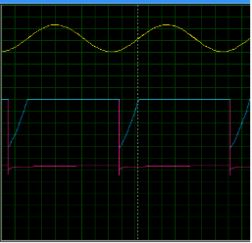
\includegraphics[scale = 1]{figuras/Simulacao_Dimmer}
				\caption{Exemplo de circuito dimmer entrada, pulso e saída.}
			\end{center}
		\end{figure}

 		\begin{figure}[H]
 			\begin{center}
 				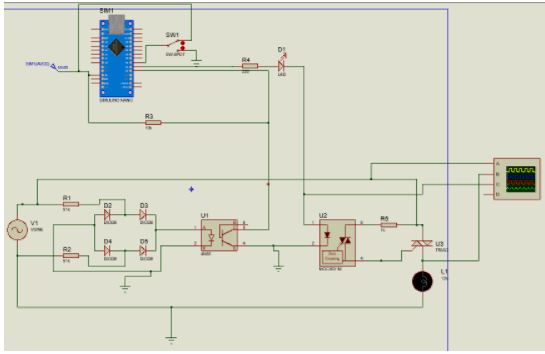
\includegraphics[scale = 1]{figuras/Circuito_Dimmer}
 				\caption{Exemplo de circuito dimmer entrada, pulso e saída.}
 			\end{center}
 		\end{figure}
 		
 		 		\begin{figure}[H]
 		 			\begin{center}
 		 				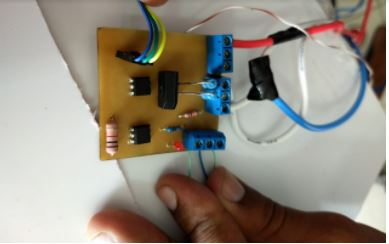
\includegraphics[scale = 1]{figuras/PCB_DImmer}
 		 				\caption{Exemplo de circuito dimmer entrada, pulso e saída.}
 		 			\end{center}
 		 		\end{figure}
 		 		
 O circuito de dimmer mostrou resultados satisfatórios quando conectado a rede elétrica e a uma lâmpada para verificar seu funcionamento através da intensidade luminosa, já que não dispunhamos de um cabo atenuador de tensão para o osciloscópio.
 
 Utilizando o multímetro digital MINIPA fomos capazes de observar que a tensão aumentava de acordo com o valor setado pelo microcontrolador, variando entre 0V e 216V, o sistema também foi capaz de dar a partida suave no motor, porém quando o sistema foi desligado o motor gerou uma corrente reversa que acabou por danificar o sistema.
 
\subsection{Inversor}
Inversores são conversores estáticos que, segundo Matakas Jr. E Komatsu (2011) transformam corrente ou tensão de forma contínua para a alternada. Muitos equipamentos operam em corrente/tensão contínua, sendo que a rede elétrica opera em corrente/tensão contínua. Portanto, a maneira mais simples de se trabalhar sem necessidade de mudanças drásticas em nenhum dos dois sistemas é se utilizar um inversor.

Este equipamento pode ser monofásico ou trifásico, sendo que o modelo utilizado no projeto será monofásico, e irá converter 12V da bateria que alimenta o sistema para 220V, valor de tensão que os outros componentes do sistema trabalham. Neste caso, com apenas duas chaves eletrônicas e uma fonte de tensão CC dividida é possível obter o inversor desejado.

Os inversores podem operar com duas tecnologias, senóide modificada ou senóide pura. No primeiro caso, formam uma onda quadrática, aproximando-se da senoidal AC, bom custo x benefício e pode ser aplicado na maioria dos casos, exceto para motores. O segundo caso pode ser usado como suprimento de energia AC em qualquer sistema, o que difere é o valor e o tamanho.

Um inversor bem dimensionado tem a potência maior que o consumo dos equipamentos para evitar que este trabalhe sempre em máxima potência,em suma um inversor é projetado em 3 estágios, oscilador, driver de corrente e transformador.
\begin{figure}[H]
	\begin{center}
		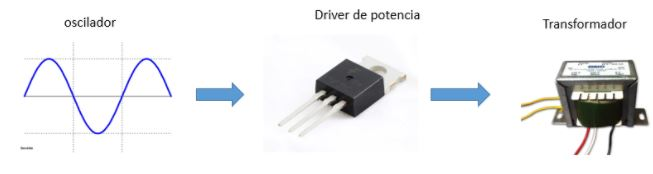
\includegraphics[scale = 0.75]{figuras/dim_inversor.JPG}
		\caption{ Diagrama Elétrico Preliminar}
	\end{center}
\end{figure}

Em primeiro lugar o oscilador transforma a corrente contínua em uma onda quadrada de 60Hz, que precisa ser adequada para uma onda senoidal, para isso é utilizado um filtro passa faixa centrado em 60Hz para eliminar as harmônicas indesejadas e obter uma onda senoidal mais eficaz possível. Entretanto, a saída do oscilador possui uma corrente muito baixa, por isso é necessário um ganho de corrente, para que seja entregue uma potência satisfatória na entrada do primário do transformador. Como a potência requerida é muito alta, se faz necessário que sejam inseridos vários transistores em paralelo para aumentar o ganho de corrente.

Na última fase o transformador faz a elevação da tensão para 220V que é a tensão necessária para ligar o compressor.

\subsection{Oscilador de onda quadrada}
Para que o inversor possa partir de uma corrente DC e por fim passe por um transformador para que seja elevada, é necessário que haja uma oscilação entre as entradas do transformador, a maneira mais viável de realizar essa oscilação é criando duas ondas quadradas defasadas em exatamente $180^o$.

Para criar as duas ondas de oscilação defasadas em $180^oC$ e quadradas, foram escolhidos os circuitos 555 no modo astável e um flip-flop tipo D, como desejamos uma saída de 120Hz para que sua borda de subida provoque uma oscilação de 60Hz nos flip flops.

Para que a frequência do CI 555 fica-se centrada em 60Hz foi utilizado o circuito no modo astável, onde um divisor resistivo entre os pinos threshold(6) discharge(7) e o capacitor de trigger(2) determinam a frequência de saída de acordo com a seguinte equação:

$$
f = \frac{1,44}{(R_1+2R_2)\times C}
$$

Onde $R_1$ é o resistor entre os pinos 6 e 7 $R_2$ é o resistor entre os pinos 6 e 2 e C é a capacitância do capacitor entre o pino 2 e o GND do circuito Arbitramos um capacitor comercial de 22uF e um resistor de baixo valor 100$\Omega$ para $R_1$ e calculamos o outro valor e obtemos um valor de 330 $\Omega$ no resistor $R_2$.

A saída do circuito 555 que corresponde a uma onda quadrada de 120Hz é conectada a um flip flop tipo D com saida Q e Q  barrado realizamos uma conexão da entrada de dados com a saída de Q dessa forma temos um loop infinito entre 0 e 1 afinal o dado de Q passa para Q barrado e assim por diante eternamente, criando duas saídas defasadas uma da outra, o circuito simulado no software proteus 8.0.

Foi escolhido utilizar um flip flop tipo D HEF4013 que apresenta uma defasagem entre Q e Q barrado de 200uS desta forma podemos utilizar esse chip para implementar o tempo morto do sistema, ou seja, um tempo de segurança para evitar que as duas ondas entrem em funcionamento causando um curto circuito nos transistores levando a sua danificação.

\begin{figure}[H]
	\begin{center}
		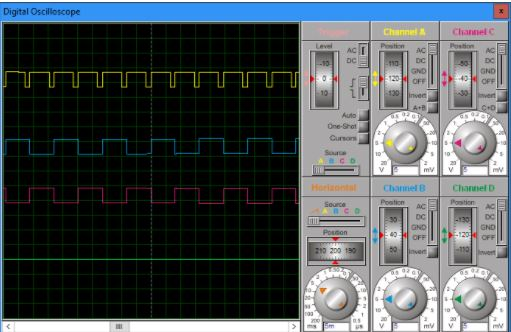
\includegraphics[scale = 0.75]{figuras/Simulacao_FlipFlop}
		\caption{ Simulação do Oscilador com proteus 8.0.}
	\end{center}
\end{figure}

Onde o canal 1 representa a saída do circuito 555, ou seja, a entrada do clock do circuito flip flop, e os canais 2 e 3 representam as duas saídas do flip flip.
\begin{figure}[H]
	\begin{center}
		\includegraphics[scale = 0.75]{figuras/FlipFlop}
		\caption{ Simulação do Oscilador com proteus 8.0.}
	\end{center}
\end{figure}

\subsection{Transformador}
O transformador utilizado nos testes possui os seguintes dados:
\begin{itemize}
	\item Tensão de Entrada: 12 Volts;
	\item Tensão de Saída: 220 Volts;
	\item Corrente de Saída: 5 Amperes.
	\end{itemize}
	
	Para dimensioná-lo  foram realizados alguns cálculos de características importantes, os quais são demonstrados os resultados abaixo:
	\begin{itemize}
		\item Potência de Saída: 1100 Watts
		\item Seção do Núcleo: 3979 $mm^2$
		\item Carretel: 50 X 80 (seção: 4000 $mm^2$)
		\item Chapa: 50 mm
		\item Empilhamento: 80 mm
		\item Espiras/volt: 15.015015015015
		\item Espiras no Enrolamento Primário: 180.18018018018
		\item Espiras no Enrolamento Secundário: 3468.46846846847
		\item Corrente no Enrolamento Primário: 33.4782608695652 Ampéres
		\item Potência no Enrolamento Primário: 401.739130434783 Watts
		\item Densidade de corrente: 2.2 A/$mm^2$
		\item Seção do fio Primário : 15.2173913043478 $mm^2$
		\item Seção do fio Secundário : 2.27272727272727 $mm^2$
		\item Fio do Primário: 6 AWG (Diâmetro: 4.1 - Secção 13 $mm^2$)
		\item Fio do Secundário: 15 AWG (Diâmetro: 1.5 - Secção 1.7 $mm^2$)
		
	\end{itemize}
	
	Cálculo de ajuste para montagem:
	\begin{itemize}
		\item Fio do Primário: 8 AWG (Diametro: 3.3 - Secção 8.4 $mm^2$)
		\item Fio do Secundário: 18 AWG (Diametro: 1 - Secção 0.82 $mm^2$)
		
	\end{itemize}
	
A montagem sugerida acima não é comercializada, portanto realizou-se uma montagem sob medida,a figura abaixo, apresenta este transformador.
	
	\begin{figure}[H]
		\begin{center}
			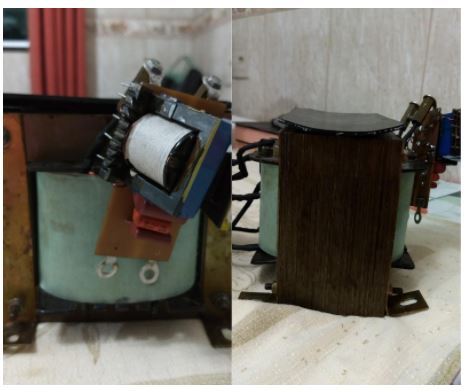
\includegraphics[scale = 0.75]{figuras/Transformador}
			\caption{ Simulação do Oscilador com proteus 8.0.}
		\end{center}
	\end{figure}
	
	
	Uma consequência da utilização desse transformador seria o aumento do peso do sistema de maneira considerável. Sendo assim, pelo fato de um dos requisitos do sistema ser a mobilidade da transportadora de órgãos, sua utilização prejudicaria este requisito, tornando-se praticamente inviável.
	
	\subsection{Filtro de 60Hz}
	Foi utilizado um filtro LC para filtrar os harmônicos indesejados e deixar o circuito o mais otimizado possível para 60Hz, setando a frequência de ressonância do circuito em 60Hz. Os filtros RC e RLC foram descartados pois estes dissiparam muita potência devido a presença do resistir como existe uma grande dificuldade em encontrar indutores apropriados para alta tensão, foram confeccionados indutores para o maior valor de indutância possível e que fossem de um tamanho que não compromete-se a viabilidade do sistema, desta forma conseguimos obter um valor de indutância de 1,4uH.
	
	A equação do filtro passa baixa com RL é a seguinte:
	\begin{equation}
	f_c = \frac{1}{2 \times \pi \times sqrt{L\times C}}
	\end{equation}
	
	Onde $f_c$ é frequência de corte L é a indutância e C é a capacitância do circuito, assim calculando, é necessário um capacitor de 5.03uF para uma frequência de corte de 60Hz.
	
	\subsection{Driver de Potência}
	Em primeiro lugar foi utilizado um buffer e amplificador com transistores TBJ tipo TIP41 para isolar o circuito oscilador do driver de potência e evitar danos da parte de baixa corrente para a parte de alta corrente, como estamos trabalhando com ondas quadradas os transistores são mantidos em saturação durante todo o tempo, afinal a tensão do coletor é muito alta em relação a tensão do source, dessa forma o transistor atua em modo de saturação.
	
	Essa mesma saída entra em um banco de transistores de potência com o transistor IRFZ3205 que possui tensão de gate source Vgs de 20V e tensão Vds de 55V máximo, capacidade de suportar corrente de Igs de até 100A e capacidade de dissipação de potência de até 200W, por este motivo escolhemos este transistor em especial, pois este seria o melhor e mais viável modelo comercial para suportar altas correntes, afinal para acionar um motor de indução de 1/10HP, que apresentou tensão de pico de 4.8A medidos com alicate amperímetro através de uma partida direta é necessário uma corrente de 88A na entrada do transformador, desprezando as perdas do transformador.
	
	A valor da corrente para cada transistor é dado pela corrente total dividida pelo número de transistores que são colocados em paralelo, em cada lado do circuito, dessa forma utilizamos 7 transistores de cada lado para que pudéssemos tem uma dissipação máxima de 1400W potência suficiente para ligar o motor de 1/10HP, sem exigir muito das características do transistor evitando o seu aquecimento.
	
		\begin{figure}[H]
			\begin{center}
				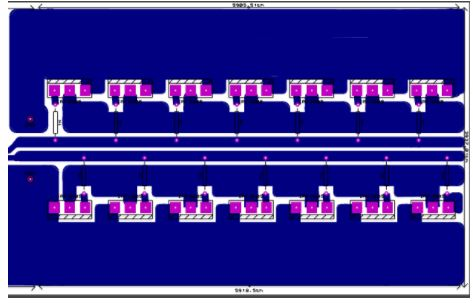
\includegraphics[scale = 0.75]{figuras/Layout_Potencia}
				\caption{  Layout do banco de potência.}
			\end{center}
		\end{figure}
